\documentclass{article}
\usepackage{tikz}
\usepackage{amssymb}
\usetikzlibrary{shapes.geometric, arrows.meta, positioning}

\tikzset{
  startstop/.style={rectangle, rounded corners, minimum width=3cm, minimum height=1cm, text centered, draw=black, fill=red!30},
  io/.style={trapezium, trapezium stretches=true, trapezium left angle=70, trapezium right angle=110, minimum width=3cm, minimum height=1cm, align=center, text centered, draw=black, fill=blue!30},
  process/.style={rectangle, minimum width=3cm, minimum height=1cm, text centered, text width=3cm, draw=black, fill=orange!30},
  decision/.style={diamond, aspect=1.5, minimum width=3cm, minimum height=1cm, text centered, draw=black, fill=green!30},
  arrow/.style={thick, ->, >=stealth}
}

\title{Flowcharts}
\author{Gabriele Fonzar}
\pagestyle{empty}

\begin{document}

\maketitle
\thispagestyle{empty}

\section{Exercise 1}

\begin{center}
\makebox[\textwidth][c]{%
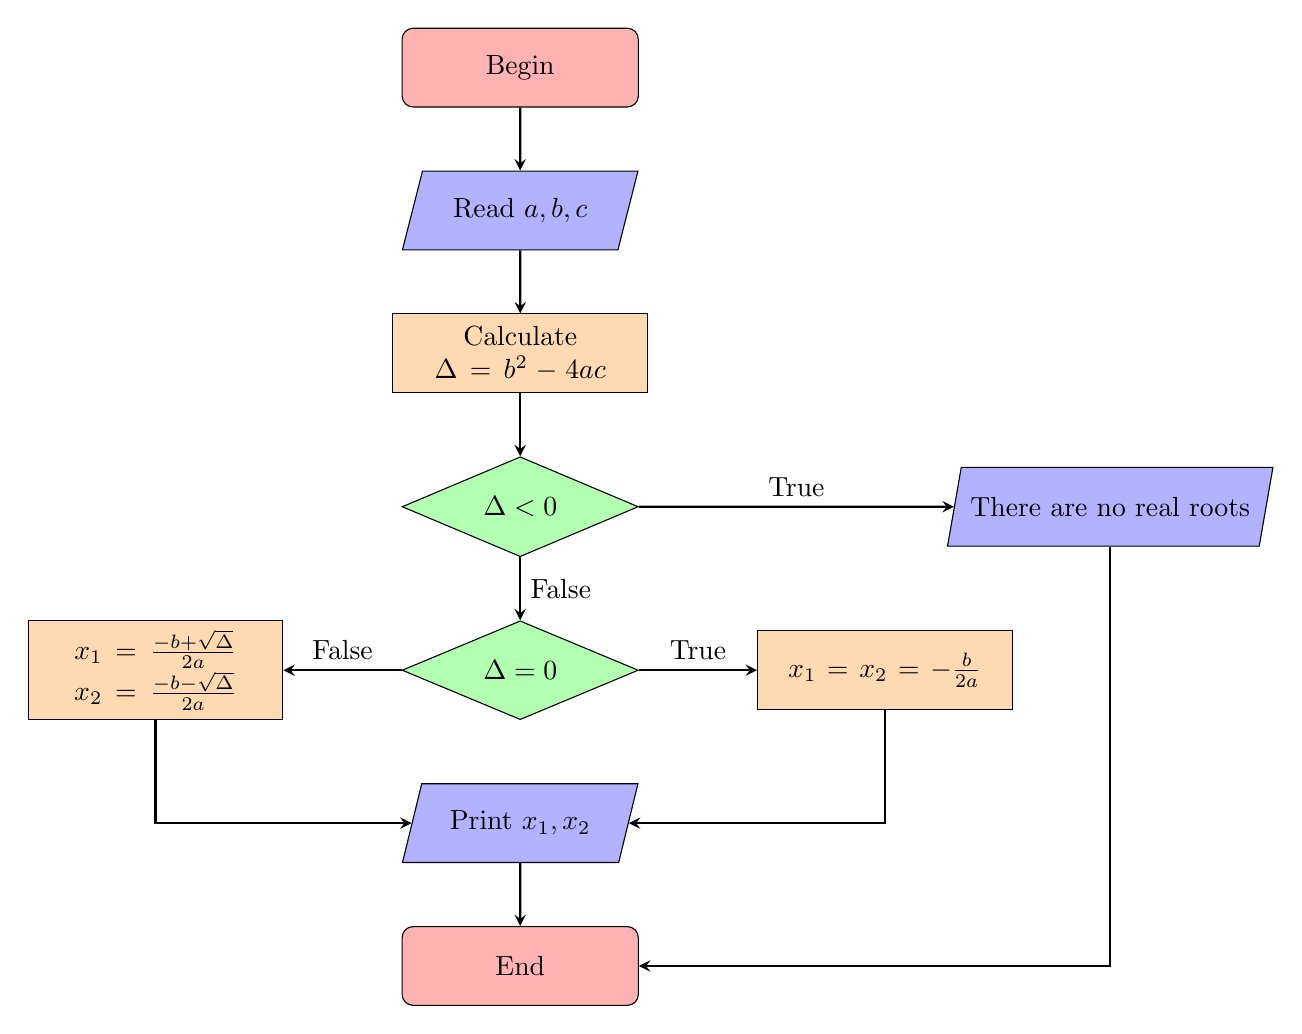
\begin{tikzpicture}[node distance=0.8cm and 1.5cm]

  \node (start) [startstop] {Begin};
  \node (input) [io, below=of start] {Read $a, b, c$};
  \node (process1) [process, below=of input] {Calculate $\Delta=b^2-4ac$};
  \node (decision1) [decision, below=of process1] {$\Delta < 0$};
  \node (output1) [io, right=4cm of decision1] {There are no real roots};
  \node (decision2) [decision, below=of decision1] {$\Delta = 0$};
  \node (output2) [process, right=of decision2] {$x_1 = x_2 = - \frac{b}{2a}$};
  \node (output3) [process, left=of decision2] {$x_1 = \frac{-b+\sqrt{\Delta}}{2a}$ \\ $x_2 = \frac{-b-\sqrt{\Delta}}{2a}$};
  \node (output) [io, below=of decision2] {Print $x_1, x_2$};
  \node (stop) [startstop, below=of output] {End};
  
  \draw [arrow] (start) -- (input);
  \draw [arrow] (input) -- (process1);
  \draw [arrow] (process1) -- (decision1);
  \draw [arrow] (decision1) -- node[right] {False} (decision2);
  \draw [arrow] (decision1) -- node[above] {True} (output1);
  \draw [arrow] (decision2) -- node[above] {False} (output3);
  \draw [arrow] (decision2) -- node[above] {True} (output2);
  \draw [arrow] (output1) |- (stop);
  \draw [arrow] (output) -- (stop);
  \draw [arrow] (output2) |- (output);
  \draw [arrow] (output3) |- (output);

\end{tikzpicture}
}
\end{center}


\section{Exercise 2}

\begin{center}
\makebox[\textwidth][c]{%
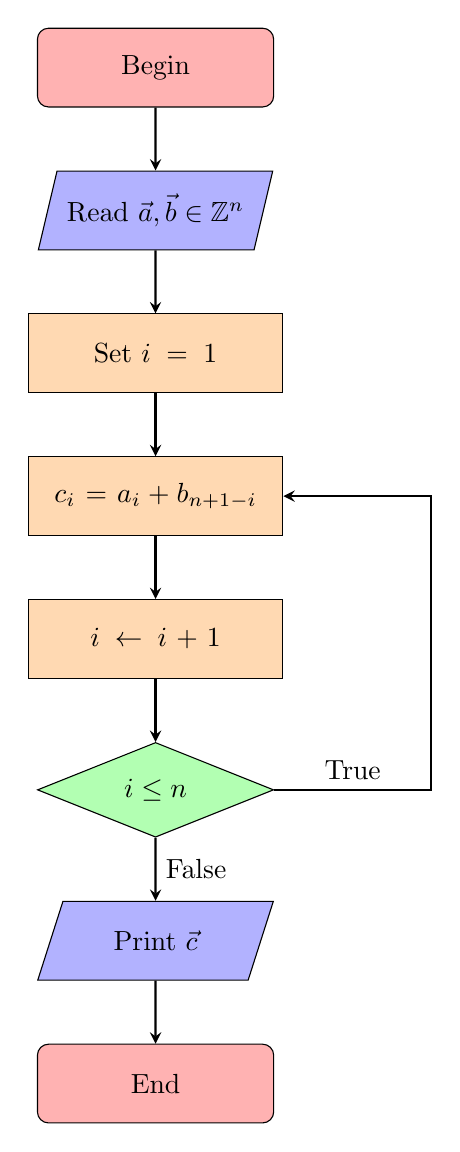
\begin{tikzpicture}[node distance=0.8cm and 1.5cm]

  \node (start) [startstop] {Begin};
  \node (input) [io, below=of start] {Read $\vec{a}, \vec{b} \in \mathbb{Z}^n$};
  \node (process) [process, below=of input] {Set $i=1$};
  \node (process1) [process, below=of process] {$c_i = a_i + b_{n+1-i}$};
  \node (process2) [process, below=of process1] {$i \leftarrow i+1$};
  \node (decision1) [decision, below=of process2] {$i \leq n$};
  \node (output) [io, below=of decision1] {Print $\vec{c}$};
  \node (stop) [startstop, below=of output] {End};
  
  \draw [arrow] (start) -- (input);
  \draw [arrow] (input) -- (process);
  \draw [arrow] (process) -- (process1);
  \draw [arrow] (process1) -- (process2);
  \draw [arrow] (process2) -- (decision1);
  \draw [arrow] (decision1) -- node[right] {False} (output);
  \draw [arrow] (decision1) -- node[above] {True} ++(3.5cm,0) |- (process1);
  \draw [arrow] (output) -- (stop);

\end{tikzpicture}
}
\end{center}



\section{Exercise 3}

\begin{center}
\makebox[\textwidth][c]{%
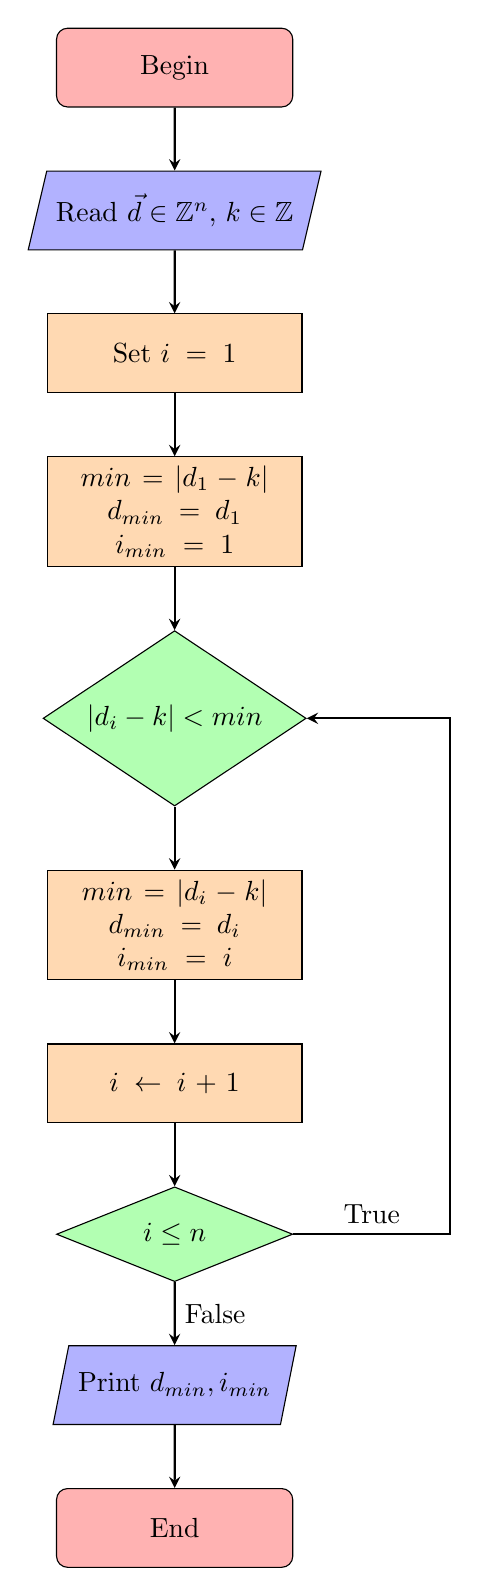
\begin{tikzpicture}[node distance=0.8cm and 1.5cm]

  \node (start) [startstop] {Begin};
  \node (input) [io, below=of start] {Read $\vec{d} \in \mathbb{Z}^n$, $k \in \mathbb{Z}$};
  \node (process) [process, below=of input] {Set $i=1$};
  \node (process1) [process, below=of process] {$min = |d_1 - k|$ \\ $d_{min} = d_1$ \\ $i_{min} = 1$};
  \node (decision1) [decision, below=of process1] {$|d_i - k| < min$};
  \node (process2) [process, below=of decision1] {$min = |d_i - k|$ \\ $d_{min} = d_i$ \\ $i_{min} = i$};
  \node (process3) [process, below=of process2] {$i \leftarrow i+1$};
  \node (decision2) [decision, below=of process3] {$i \leq n$};
  \node (output) [io, below=of decision2] {Print $d_{min}, i_{min}$};
  \node (stop) [startstop, below=of output] {End};
  
  \draw [arrow] (start) -- (input);
  \draw [arrow] (input) -- (process);
  \draw [arrow] (process) -- (process1);
  \draw [arrow] (process1) -- (decision1);
  \draw [arrow] (decision1) -- (process2);
  \draw [arrow] (process2) -- (process3);
  \draw [arrow] (process3) -- (decision2);
  \draw [arrow] (decision2) -- node[right] {False} (output);
  \draw [arrow] (decision2) -- node[above] {True} ++(3.5cm,0) |- (decision1);
  \draw [arrow] (output) -- (stop);

\end{tikzpicture}
}
\end{center}


\section{Exercise 4}

\begin{center}
\makebox[\textwidth][c]{%
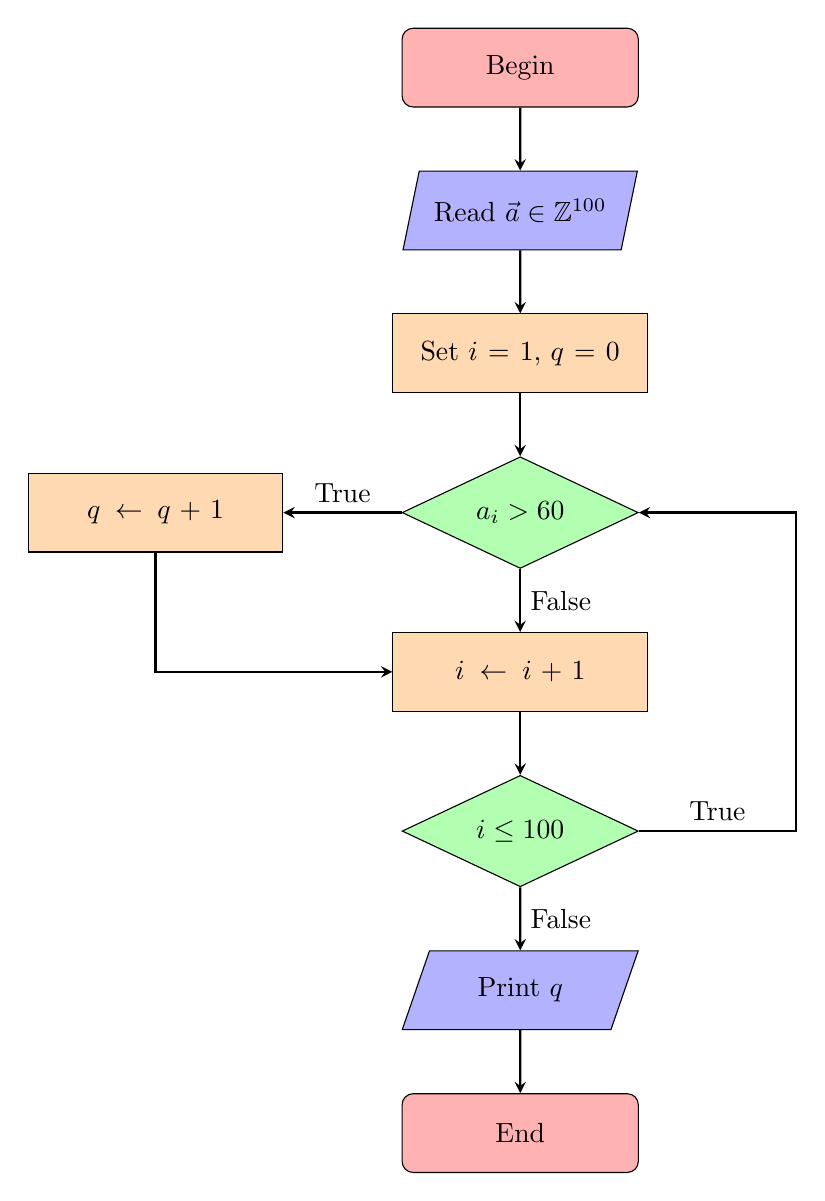
\begin{tikzpicture}[node distance=0.8cm and 1.5cm]

  \node (start) [startstop] {Begin};
  \node (input) [io, below=of start] {Read $\vec{a} \in \mathbb{Z}^{100}$};
  \node (process) [process, below=of input] {Set $i=1$, $q=0$};
  \node (decision1) [decision, below=of process] {$a_i > 60$};
  \node (process3) [process, below=of decision1] {$i \leftarrow i+1$};
  \node (process2) [process, left=of decision1] {$q \leftarrow q+1$};
  \node (decision2) [decision, below=of process3] {$i \leq 100$};
  \node (output) [io, below=of decision2] {Print $q$};
  \node (stop) [startstop, below=of output] {End};
  
  \draw [arrow] (start) -- (input);
  \draw [arrow] (input) -- (process);
  \draw [arrow] (process) -- (decision1);
  \draw [arrow] (decision1) -- node[above] {True} (process2);
  \draw [arrow] (process2) |- (process3);
  \draw [arrow] (decision1) -- node[right] {False} (process3);
  \draw [arrow] (process3) -- (decision2);
  \draw [arrow] (decision2) -- node[right] {False} (output);
  \draw [arrow] (decision2) -- node[above] {True} ++(3.5cm,0) |- (decision1);
  \draw [arrow] (output) -- (stop);

\end{tikzpicture}
}
\end{center}

\section{Exercise 5}

\begin{center}
\makebox[\textwidth][c]{%
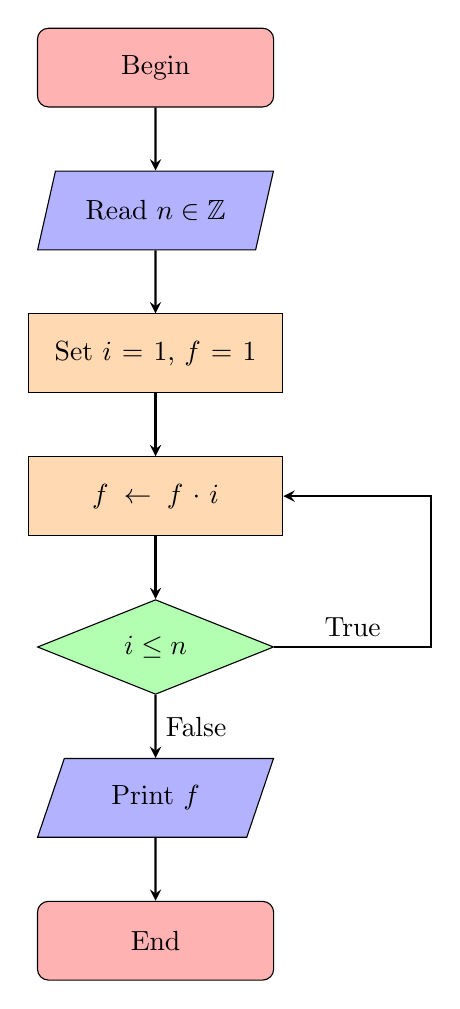
\begin{tikzpicture}[node distance=0.8cm and 1.5cm]

  \node (start) [startstop] {Begin};
  \node (input) [io, below=of start] {Read $n \in \mathbb{Z}$};
  \node (process) [process, below=of input] {Set $i=1$, $f=1$};
  \node (process2) [process, below=of process] {$f \leftarrow f \cdot i$};
  \node (decision2) [decision, below=of process2] {$i \leq n$};
  \node (output) [io, below=of decision2] {Print $f$};
  \node (stop) [startstop, below=of output] {End};
  
  \draw [arrow] (start) -- (input);
  \draw [arrow] (input) -- (process);
  \draw [arrow] (process) -- (process2);
  \draw [arrow] (process2) -- (decision2);
  \draw [arrow] (decision2) -- node[right] {False} (output);
  \draw [arrow] (decision2) -- node[above] {True} ++(3.5cm,0) |- (process2);
  \draw [arrow] (output) -- (stop);

\end{tikzpicture}
}
\end{center}



\end{document}
